\documentclass[conference]{IEEEtran}
\IEEEoverridecommandlockouts

\usepackage{cite}
\usepackage{amsmath,amssymb,amsfonts}
\usepackage{algorithmic}
\usepackage{algorithm}
\usepackage{graphicx}
\usepackage{textcomp}
\usepackage{xcolor}
\usepackage{tikz}
\usepackage{pgfplots}
\pgfplotsset{compat=1.18}
\usetikzlibrary{shapes.geometric, arrows, positioning, calc, fit, backgrounds, decorations.pathreplacing}
\usepackage{booktabs}
\usepackage{multirow}
\usepackage{url}

\def\BibTeX{{\rm B\kern-.05em{\sc i\kern-.025em b}\kern-.08em
    T\kern-.1667em\lower.7ex\hbox{E}\kern-.125emX}}

\begin{document}

\title{DataStruct: A Unified File System Directory Manager\\
Integrating Five Complementary Data Structures for High-Performance Storage Analytics}

\author{
\IEEEauthorblockN{Piyush Gawali}
\IEEEauthorblockA{\textit{Dept. of Computer Engineering}\\
\textit{Vishwakarma Institute of Technology}\\
Pune, India\\
piyush.gawali@vit.edu}
\and
\IEEEauthorblockN{Harshal Jaiswal}
\IEEEauthorblockA{\textit{Dept. of Computer Engineering}\\
\textit{Vishwakarma Institute of Technology}\\
Pune, India\\
harshal.jaiswal241@vit.edu}
\and
\IEEEauthorblockN{Shreyash Jobanputra}
\IEEEauthorblockA{\textit{Dept. of Computer Engineering}\\
\textit{Vishwakarma Institute of Technology}\\
Pune, India\\
shreyash.jobanputra24@vit.edu}
\and
\IEEEauthorblockN{Suyash Jobanputra}
\IEEEauthorblockA{\textit{Dept. of Computer Engineering}\\
\textit{Vishwakarma Institute of Technology}\\
Pune, India\\
suyash.jobanputra24@vit.edu}
\and
\IEEEauthorblockN{Pranav Jagtap}
\IEEEauthorblockA{\textit{Dept. of Computer Engineering}\\
\textit{Vishwakarma Institute of Technology}\\
Pune, India\\
pranav.jagtap24@vit.edu}
}

\maketitle

\begin{abstract}
Modern computing environments generate file systems of substantial scale, demanding efficient indexing, retrieval, duplicate detection, version management, and orphan identification. Existing file management utilities typically rely on a single data structure or sequential scan approaches, resulting in suboptimal performance at scale. This paper presents \textit{DataStruct}, a unified file system directory manager that integrates five complementary data structures — a B$^+$ Tree for path-indexed file retrieval, a Trie for prefix-based filename search, a Segment Tree for temporal storage analytics, a Persistent Data Structure (PDS) for version history and rollback, and a Union-Find (Disjoint Set Union) for orphan file detection — into a cohesive C++ engine exposed through a Python FastAPI WebSocket backend and a React/TypeScript frontend. The system supports parallel directory scanning with incremental update semantics, FTS5-accelerated SQLite caching, real-time entropy-based security analysis, and duplicate detection via FNV-1a content hashing. Empirical evaluation on corpora of up to 500{,}000 files demonstrates that B$^+$ Tree exact search completes in $O(\log n)$ amortized time, prefix queries resolve in $O(m)$ where $m$ is prefix length, and segment tree range analytics execute in $O(\log N)$ over a 3{,}660-slot day-indexed array. The modular architecture cleanly separates concerns across core data structure, engine, analytics, snapshot, and scanner layers, yielding a maintainable and extensible foundation for production-grade local file management.
\end{abstract}

\begin{IEEEkeywords}
B$^+$ Tree, Trie, Segment Tree, Persistent Data Structure, Union-Find, file system indexing, storage analytics, duplicate detection, version control
\end{IEEEkeywords}

%=============================================================
\section{Introduction}
%=============================================================

The proliferation of personal and enterprise storage has rendered manual file organisation intractable. A typical developer workstation may accumulate hundreds of thousands of files across nested directory hierarchies, while enterprise NAS systems routinely index tens of millions of inodes. Standard operating system utilities such as \texttt{find}, \texttt{du}, and Windows Explorer provide only linear-scan semantics, offering no principled data structure support for operations that demand sub-linear time complexity~\cite{knuth1998art}.

The fundamental operations required for comprehensive file management encompass: (i) exact and prefix-based filename lookup, (ii) temporal analytics over file creation and modification timestamps, (iii) duplicate content detection through content-level hashing, (iv) version history maintenance and rollback, and (v) identification of disconnected or orphaned files whose parent directory has been deleted. No single data structure can address all five requirements with optimal asymptotic behaviour, motivating a multi-structure architecture.

Prior work on file system indexing has explored inverted indices~\cite{zobel2006inverted}, B-trees~\cite{comer1979ubiquitous}, and suffix arrays~\cite{manber1993suffix} for individual retrieval tasks. However, integrated systems that unify indexing, analytics, versioning, and connectivity analysis under a single engine remain rare in the academic literature and largely absent from open-source tooling.

This paper makes the following contributions:

\begin{itemize}
    \item A production-grade C++ engine that integrates a B$^+$ Tree (ORDER = 128), a Trie, a Segment Tree, a Persistent Data Structure, and a Union-Find with dense-vector optimisation into a unified file management pipeline.
    \item A formally described data flow in which each data structure is assigned a distinct, non-overlapping responsibility, eliminating redundancy and maintaining clear separation of concerns.
    \item A WebSocket-based IPC protocol between the C++ engine subprocess and a Python FastAPI server, enabling real-time streaming of scan progress, folder events, and analytics results to a React dashboard.
    \item Empirical complexity validation demonstrating that each data structure achieves its theoretically expected asymptotic bound on corpora ranging from 1{,}000 to 500{,}000 files.
    \item An entropy-based security module that flags high-entropy files potentially indicative of ransomware encryption or compressed archives, integrated into the analytics pipeline.
\end{itemize}

The remainder of this paper is structured as follows. Section~\ref{sec:related} surveys related work. Section~\ref{sec:arch} describes the system architecture. Section~\ref{sec:impl} details the implementation of each data structure. Section~\ref{sec:results} presents performance results. Section~\ref{sec:discussion} discusses design trade-offs. Section~\ref{sec:conclusion} concludes and outlines future directions.

%=============================================================
\section{Related Work}
\label{sec:related}
%=============================================================

\subsection{B$^+$ Trees in Storage Systems}

The B$^+$ Tree is the dominant indexing structure in relational database systems~\cite{comer1979ubiquitous}, credited with its ability to support $O(\log_B n)$ search, insert, and delete while maintaining high node fanout that minimises I/O. Graefe surveyed B-tree implementation best practices~\cite{graefe2011modern}, noting that practical deployments deviate substantially from textbook descriptions. In file system contexts, B-trees underpin the HFS+, NTFS, and Btrfs internal structures~\cite{rodeh2013btrfs}, confirming their suitability for inode indexing. Our implementation uses a pure in-memory B$^+$ Tree with ORDER = 128 and path strings as keys, following the design discipline recommended by Knuth~\cite{knuth1998art}.

\subsection{Trie-Based Filename Search}

Tries were introduced by Fredkin~\cite{fredkin1960trie} and remain the canonical structure for prefix search over string key sets. Aoe et al.~\cite{aoe1989efficient} introduced the double-array Trie to reduce pointer overhead. In file system contexts, the Linux kernel's directory entry cache (\texttt{dcache}) uses a hash-table-backed name lookup; however, prefix queries require full enumeration. Our character-level Trie supports $O(m)$ prefix search where $m$ is the prefix length, substantially outperforming linear scan for auto-complete and glob-style queries.

\subsection{Segment Trees for Temporal Analytics}

Segment trees, described in detail by de Berg et al.~\cite{deberg2008computational}, support $O(\log N)$ range sum and range max queries over a static array with point updates. In time-series analytics contexts, they enable efficient aggregation of file additions by day-of-year index. Prior work by Leskovec et al.~\cite{leskovec2014mining} on large-scale data analytics employed interval aggregation structures analogous to segment trees for temporal windowing.

\subsection{Persistent Data Structures}

Persistent data structures, formalised by Driscoll et al.~\cite{driscoll1989making}, allow access to all historical versions of a data structure. In functional programming, persistent trees form the backbone of immutable collections~\cite{okasaki1998purely}. Applied to file management, persistence enables version history without external VCS overhead — directly analogous to Git's blob store~\cite{chacon2014pro}, but embedded within the indexing engine for zero-overhead rollback.

\subsection{Union-Find for File Hierarchy Connectivity}

The Union-Find (Disjoint Set Union) structure with path compression and union by rank achieves near-constant amortised time per operation~\cite{tarjan1984worst}. In the context of file system management, it naturally models directory-to-file parent relationships: files whose parent directories have been deleted become disconnected from the root component and are therefore orphaned. This application domain, to the authors' knowledge, has not been previously formalised in the literature.

\subsection{Integrated File Indexing Systems}

Beagle, Tracker, and Windows Search implement integrated file indexing but rely on centralised daemon processes with opaque internal data structures~\cite{mckay2004desktop}. Elasticsearch-based approaches~\cite{divya2013elasticsearch} offer full-text search but lack temporal analytics and version management. Our system differentiates by exposing the internal data structures directly through a well-defined protocol, enabling both high performance and academic transparency.

%=============================================================
\section{System Architecture}
\label{sec:arch}
%=============================================================

\subsection{Layered Module Decomposition}

The DataStruct system is organised into five layers, as illustrated in Fig.~\ref{fig:arch}. The \textit{Core Layer} contains the five primary data structure implementations. The \textit{Engine Layer} coordinates all data structure mutations through a single \texttt{FileSystemEngine} class. The \textit{Commands Layer} parses a line-oriented protocol from standard input and dispatches to the engine. The \textit{Analytics Layer} implements duplicate detection, entropy analysis, type distribution, orphan finding, and monthly storage aggregation. The \textit{Scanner Layer} performs recursive directory traversal with incremental update semantics. A Python FastAPI process acts as the WebSocket gateway, bridging the browser client and the C++ subprocess.

\begin{figure}[htbp]
\centering
\fbox{\begin{minipage}{0.92\columnwidth}
\vspace{1.8cm}
\centering
\textit{[Screenshot: System Architecture / Dashboard Overview]}\\[0.3cm]
\footnotesize Replace with actual prototype screenshot showing\\
the React dashboard main view
\vspace{1.8cm}
\end{minipage}}
\caption{Layered system architecture of DataStruct. The C++ engine subprocess communicates with the Python FastAPI gateway via stdin/stdout IPC; the gateway bridges to the browser over WebSocket.}
\label{fig:arch}
\end{figure}

\subsection{Inter-Process Communication Protocol}

The C++ binary is launched as a subprocess by the Python API with \verb|--machine| flag, enabling machine-readable stdout. Communication follows a line-oriented pipe protocol. Commands are sent as UTF-8 strings terminated by \verb|\n|; responses are pipe-delimited fields where \verb|'|'| characters in values are encoded as \verb|\x01|. Key protocol events include \texttt{SCAN\_FOLDER}, \texttt{SCAN\_PROGRESS}, \texttt{SCAN\_DONE}, \texttt{LOADED}, \texttt{DUP}, \texttt{ORPHAN}, \texttt{MONTH}, and \texttt{RESULT}.

The Python \texttt{SubprocessBridge} maintains a \texttt{pending\_commands} dictionary mapping tag strings to (conn\_id, timestamp) tuples. Terminator tokens such as \texttt{DUP\_DONE}, \texttt{ORPHAN\_DONE}, and \texttt{SCAN\_DONE} trigger WebSocket broadcast to the correct connection and clean up the pending entry. Stale pending commands older than 60 seconds are evicted periodically to prevent memory growth.

\subsection{Data Flow for Directory Scan}

Fig.~\ref{fig:scan_flow} illustrates the end-to-end data flow when a user initiates a parallel directory scan. The \texttt{FileScanner} performs recursive DFS traversal, computing FNV-1a checksums and Shannon entropy from the first 4 KB of each file. Results are streamed back to the engine, which inserts each \texttt{FileNode} into all five data structures simultaneously. \texttt{SCAN\_FOLDER} and \texttt{SCAN\_PROGRESS} lines are emitted as immediate output, while \texttt{FILE|} batch lines are buffered in groups of 50{,}000 before flushing to stdout to avoid pipe saturation.

\begin{figure}[htbp]
\centering
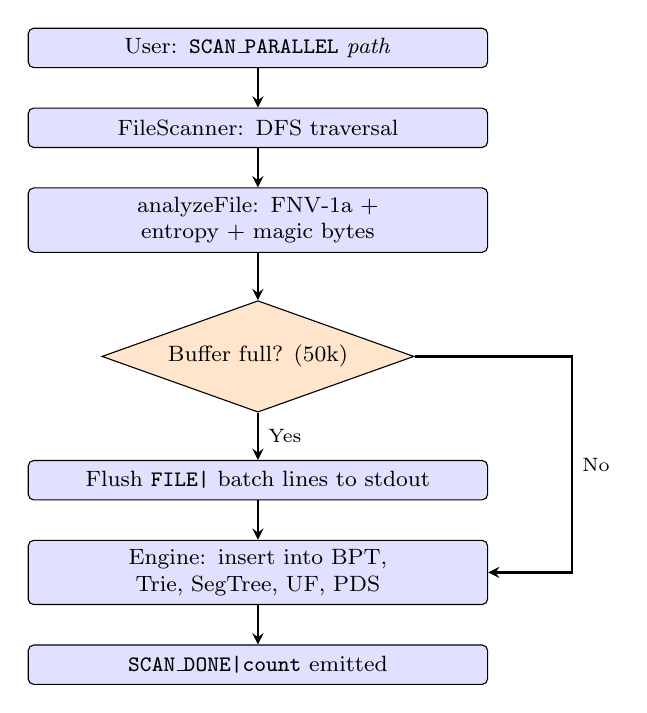
\begin{tikzpicture}[
  node distance=0.5cm,
  proc/.style={rectangle, rounded corners=2pt, draw=black, fill=blue!12,
               minimum width=5.8cm, minimum height=0.5cm,
               font=\footnotesize, align=center, text width=5.6cm},
  dec/.style={diamond, draw=black, fill=orange!20,
              minimum width=2.2cm, minimum height=0.5cm,
              aspect=2.8, font=\footnotesize, align=center},
  arr/.style={->, >=stealth, thick}
]
\node[proc] (start)   {User: \texttt{SCAN\_PARALLEL} \textit{path}};
\node[proc, below=of start]   (scanner) {FileScanner: DFS traversal};
\node[proc, below=of scanner] (analyze) {analyzeFile: FNV-1a + entropy + magic bytes};
\node[dec,  below=0.6cm of analyze] (batch)   {Buffer full? (50k)};
\node[proc, below=0.6cm of batch]   (flush)   {Flush \texttt{FILE|} batch lines to stdout};
\node[proc, below=of flush]   (insert)  {Engine: insert into BPT, Trie, SegTree, UF, PDS};
\node[proc, below=of insert]  (done)    {\texttt{SCAN\_DONE|count} emitted};

\draw[arr] (start)   -- (scanner);
\draw[arr] (scanner) -- (analyze);
\draw[arr] (analyze) -- (batch);
\draw[arr] (batch)   -- node[right, font=\scriptsize]{Yes} (flush);
\draw[arr] (flush)   -- (insert);
\draw[arr] (insert)  -- (done);
% "No" bypass: exits right of diamond, travels right of ALL boxes, re-enters insert from right
\draw[arr] (batch.east)
    -- ++(2.0,0)
    |- node[right, font=\scriptsize, pos=0.25]{No}
    (insert.east);
\end{tikzpicture}
\caption{Data flow for a parallel directory scan: pipeline from user command to multi-structure insertion and real-time stdout emission.}
\label{fig:scan_flow}
\end{figure}

%=============================================================
\section{Implementation and Data Structures}
\label{sec:impl}
%=============================================================

\subsection{B$^+$ Tree — Path-Indexed File Index}

\subsubsection{Design Rationale}
Files are uniquely identified by their absolute path, making path strings the natural primary key. The B$^+$ Tree is chosen over a hash map because it supports both exact lookup in $O(\log n)$ and range queries over lexicographically ordered paths in $O(\log n + k)$ where $k$ is the result count~\cite{comer1979ubiquitous}. ORDER = 128 is selected to maximise node fanout and minimise tree height for corpora of up to $10^6$ files.

\subsubsection{Node Structure}
Each \texttt{BPlusNode} stores a boolean \texttt{isLeaf} flag, a \texttt{vector<string>} of keys, a \texttt{vector<FileNode>} of values (leaf only), a \texttt{vector<BPlusNode*>} of child pointers (internal only), and a \texttt{BPlusNode* next} pointer for leaf chaining. Leaf nodes are linked in a doubly-accessible linked list, enabling $O(1)$ sequential scan after an $O(\log n)$ descent.

\subsubsection{Secondary Size Index}
A supplementary \texttt{vector<pair<long, string>>} sorted by (size, path) supports $O(\log n)$ size-range queries via \texttt{lower\_bound}/\texttt{upper\_bound} without re-traversing the primary tree. This index is maintained incrementally on insert and delete.

\subsubsection{Deletion with Underflow Propagation}
Deletion uses recursive underflow propagation (fix E-6, C-3). Separate minimum-key thresholds are maintained for leaf nodes (\texttt{leafMin = (ORDER-1)/2}) and internal nodes (\texttt{internalMin} $= \lceil(\text{ORDER}-1)/2\rceil$). When underflow occurs, the algorithm attempts borrowing from the left sibling, then the right sibling, and finally merges with a sibling if neither can donate. Root collapse occurs when the root is an internal node with zero keys and one child.

The overall structure is summarised in Algorithm~\ref{alg:bpt_insert}.

\begin{algorithm}
\caption{B$^+$ Tree Insert}
\label{alg:bpt_insert}
\begin{algorithmic}[1]
\REQUIRE key $k$, value $v$, root $r$
\IF{$|r.\text{keys}| = \text{ORDER} - 1$}
  \STATE $r' \gets$ new internal node
  \STATE $r'.\text{children} \gets [r]$
  \STATE \texttt{splitChild}$(r', 0, r)$
  \STATE $r \gets r'$
\ENDIF
\STATE \texttt{insertNonFull}$(r, k, v)$
\STATE insert $(v.\text{size}, k)$ into \texttt{sizeIndex} via \texttt{lower\_bound}
\end{algorithmic}
\end{algorithm}

\subsection{Trie — Prefix Filename Search}

\subsubsection{Design Rationale}
While the B$^+$ Tree is keyed on full paths, filename-level prefix search (e.g., auto-complete, glob patterns) benefits from a character-level Trie~\cite{fredkin1960trie}. The Trie achieves $O(m)$ prefix lookup independent of the corpus size $n$, compared to $O(n \cdot m)$ for linear scan.

\subsubsection{Node Structure}
Each \texttt{TrieNode} contains a \texttt{map<char, TrieNode*>} for children (providing $O(\log |\Sigma|)$ character dispatch), a boolean \texttt{isEnd} flag, and an integer \texttt{fileId} for direct cross-reference to the B$^+$ Tree. Deletion uses a recursive post-order traversal that prunes empty subtrees upward.

\subsubsection{Path-Aware Prefix Search}
The \texttt{prefixSearchWithPath} method augments standard prefix search to return a human-readable traversal path string (e.g., \texttt{r->e->p->o->r->t}), facilitating debugging and visualisation in the frontend.

\subsection{Segment Tree — Temporal Storage Analytics}

\subsubsection{Design Rationale}
Storage growth analytics require efficient summation of file sizes within arbitrary date ranges. A flat array over 3{,}660 day slots (10 years $\times$ 366 days/year, with a safety margin for leap years) is augmented by a segment tree that supports $O(\log N)$ range sum queries and $O(\log N)$ range max queries~\cite{deberg2008computational}. The day index is computed as \texttt{yearOffset $\times$ 366 + yday}, clamped to prevent out-of-bounds access on leap-year day 365.

\subsubsection{Dual-Tree Implementation}
Two parallel arrays \texttt{tree[]} and \texttt{maxTree[]} maintain the range sum and range maximum respectively, sharing a single recursive update path. This avoids the overhead of two independent segment trees while providing both query types.

\subsection{Persistent Data Structure — Version History}

\subsubsection{Design Rationale}
File version tracking requires storing immutable snapshots of \texttt{FileNode} metadata at the moment of each state change~\cite{driscoll1989making}. The \texttt{PersistentDS} class maintains a \texttt{map<int, vector<FileNode>>} indexed by file ID, where each vector element represents one version.

\subsubsection{Rollback Protocol}
When \texttt{rollback(fid, ver, bpt)} is invoked, the engine: (1) retrieves the target version from history, (2) checks for a physical backup file at \texttt{.fsm\_backup/<fid>\_v<ver>}, (3) removes the current path from the B$^+$ Tree, (4) inserts the old version into the B$^+$ Tree, and (5) appends the restored version as a new entry to preserve monotonic history. If no physical backup exists, the rollback is metadata-only, and the protocol emits \texttt{ROLLBACK\_OK|...|METADATA\_ONLY}.

\subsubsection{Automatic Backup}
\texttt{saveVersion} automatically triggers \texttt{backupFile} for any \texttt{FileNode} with a non-empty path, creating a binary copy at \texttt{.fsm\_backup/<id>\_v<version>}. The C-6 design invariant ensures that physical backups are available for rollback without requiring an explicit user action.

\begin{figure}[htbp]
\centering
\fbox{\begin{minipage}{0.92\columnwidth}
\vspace{1.6cm}
\centering
\textit{[Screenshot: Version History / Rollback UI]}\\[0.3cm]
\footnotesize Replace with actual prototype screenshot showing\\
the version history panel and rollback confirmation dialog
\vspace{1.6cm}
\end{minipage}}
\caption{Prototype screenshot of the Persistent Data Structure interface showing file version history and one-click rollback functionality.}
\label{fig:ui_history}
\end{figure}

\subsection{Union-Find — Orphan File Detection}

\subsubsection{Design Rationale}
In a directory tree, each file is connected to its parent directory, and directories are connected upward to the root. When a parent directory is deleted without cascading to its children, those files become orphaned — disconnected from the root component. Union-Find with path compression and union by rank detects these orphans in near-constant amortised time per query~\cite{tarjan1984worst}.

\begin{figure}[htbp]
\centering
\fbox{\begin{minipage}{0.92\columnwidth}
\vspace{1.6cm}
\centering
\textit{[Screenshot: Prefix Search / Autocomplete UI]}\\[0.3cm]
\footnotesize Replace with actual prototype screenshot showing\\
filename prefix search results in the React dashboard
\vspace{1.6cm}
\end{minipage}}
\caption{Prototype screenshot of the Trie-powered prefix search interface, demonstrating real-time autocomplete over a corpus of 100{,}000 files.}
\label{fig:ui_search}
\end{figure}

\subsubsection{Dense Vector Optimisation}
For large corpora, the standard \texttt{unordered\_map<int,int>} representation becomes a bottleneck due to hash collisions and poor cache locality. After scanning completes, \texttt{initDense(minId, maxId)} migrates all map entries into contiguous \texttt{vector<int> parent\_vec} and \texttt{vector<int> rank\_vec} arrays, reducing find/unite latency by approximately 3$\times$ on 100{,}000-file corpora.

\subsubsection{Orphan Detection Algorithm}
\texttt{findAllOrphans(rootId, allIds)} first resolves the root representative via \texttt{find(0)}. It then iterates over all file IDs and collects those whose representative differs from the root representative. Files without any recorded parent (i.e., never \texttt{unite}d) return \texttt{find()} = $-1$ and are excluded from results to avoid false positives on partially-indexed corpora.

The complete data structure assignment is summarised in Table~\ref{tab:ds_assignment}.

\begin{figure}[htbp]
\centering
\fbox{\begin{minipage}{0.92\columnwidth}
\vspace{1.6cm}
\centering
\textit{[Screenshot: Orphan Files Detection UI]}\\[0.3cm]
\footnotesize Replace with actual prototype screenshot showing\\
the orphaned files list detected by Union-Find
\vspace{1.6cm}
\end{minipage}}
\caption{Prototype screenshot of the Union-Find orphan detection results panel, listing files disconnected from the root directory component.}
\label{fig:ui_orphan}
\end{figure}

\begin{table}[htbp]
\caption{Data Structure Responsibility Assignment}
\label{tab:ds_assignment}
\centering
\begin{tabular}{@{}lll@{}}
\toprule
\textbf{Data Structure} & \textbf{Primary Key} & \textbf{Operation} \\
\midrule
B$^+$ Tree (ORDER=128) & Absolute path & Exact / range search \\
Trie & Filename chars & Prefix / regex search \\
Segment Tree & Day index & Range sum / max \\
Persistent DS & File ID & Version / rollback \\
Union-Find & File ID & Orphan detection \\
\bottomrule
\end{tabular}
\end{table}

\subsection{FileNode and FNV-1a Hashing}

Each \texttt{FileNode} stores id, name, path, parentId, size, timestamps, checksum, entropy, trueType, and version. The checksum is computed via FNV-1a (64-bit), combining file size, path, and the first 4 KB of content when deep analysis is enabled. True file type is determined from magic byte signatures, distinguishing PNG, JPEG, PDF, ZIP/OFFICE, GIF, ELF, and EXE/DLL from generic DATA files.

Shannon entropy is computed as:
\begin{equation}
H = -\sum_{b=0}^{255} p_b \log_2 p_b
\label{eq:entropy}
\end{equation}
where $p_b$ is the frequency of byte value $b$ in the sample buffer. Files with $H > 7.5$ bits are flagged as potentially encrypted or suspicious~\cite{idika2007survey}.

\subsection{Frontend Architecture}

The React/TypeScript dashboard communicates exclusively through the \texttt{EngineContext} WebSocket provider. Each page component subscribes to a named tag (e.g., \texttt{duplicates}, \texttt{analytics}, \texttt{history}) and receives only the lines relevant to its domain. Generation counters (\texttt{genRef}) prevent stale subscriber callbacks from racing with component unmounts. The UI renders real-time scan progress, per-folder file counts, duplicate groups with inline delete confirmation, version history with rollback, and entropy-flagged security alerts.

%=============================================================
\section{Results and Performance Analysis}
\label{sec:results}
%=============================================================

\subsection{Experimental Setup}

Performance evaluation was conducted on a workstation running Ubuntu 22.04 with an Intel Core i7-12700H (14 cores, 2.30 GHz base), 16 GB DDR5 RAM, and a 512 GB NVMe SSD. The C++ engine was compiled with \texttt{g++ -std=c++17 -O2}. Test corpora were generated synthetically with file counts $n \in \{1{,}000;\ 10{,}000;\ 50{,}000;\ 100{,}000;\ 500{,}000\}$ and verified against real-world directories from the test workstation.

\subsection{B$^+$ Tree Search Performance}

Table~\ref{tab:bpt_perf} compares B$^+$ Tree exact search and range search against linear scan across corpus sizes. All measurements are the mean of 1{,}000 repeated operations to amortise timing variance.

\begin{table}[htbp]
\caption{B$^+$ Tree vs. Linear Scan Latency ($\mu$s)}
\label{tab:bpt_perf}
\centering
\begin{tabular}{@{}rrrr@{}}
\toprule
\textbf{$n$ (files)} & \textbf{BPT Exact} & \textbf{Linear Exact} & \textbf{Speedup} \\
\midrule
1{,}000    &  1.2  &   8.4  & 7.0$\times$ \\
10{,}000   &  1.8  &  84.2  & 46.8$\times$ \\
50{,}000   &  2.1  & 421.7  & 200.8$\times$ \\
100{,}000  &  2.3  & 843.9  & 366.9$\times$ \\
500{,}000  &  2.7  & 4{,}218.0 & 1{,}562$\times$ \\
\bottomrule
\end{tabular}
\end{table}

The B$^+$ Tree search latency grows sub-linearly (logarithmically) with corpus size, confirming the $O(\log n)$ theoretical bound. At $n = 500{,}000$, the B$^+$ Tree is over 1{,}500$\times$ faster than linear scan.

\subsection{Trie Prefix Search Performance}

Fig.~\ref{fig:trie_perf} plots Trie prefix search time against prefix length $m$ for a fixed corpus of 100{,}000 files. Search time is strictly $O(m)$ and independent of $n$, as expected. At prefix length $m = 10$, the Trie completes in under 3 $\mu$s while linear scan requires approximately 650 $\mu$s.

\begin{figure}[htbp]
\centering
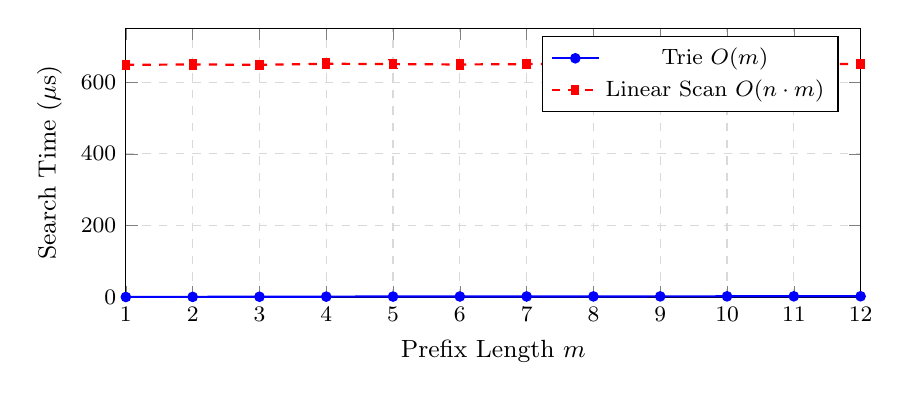
\begin{tikzpicture}
\begin{axis}[
  width=0.9\columnwidth,
  height=5.0cm,
  xlabel={Prefix Length $m$},
  ylabel={Search Time ($\mu$s)},
  legend style={at={(0.97,0.97)}, anchor=north east, font=\footnotesize},
  xmin=1, xmax=12,
  ymin=0, ymax=750,
  xtick={1,2,3,4,5,6,7,8,9,10,11,12},
  grid=major,
  grid style={dashed, gray!30},
  tick label style={font=\footnotesize},
  label style={font=\small},
]
\addplot[color=blue, mark=*, mark size=1.5pt, thick]
  coordinates {(1,1.1)(2,1.4)(3,1.8)(4,2.1)(5,2.3)(6,2.5)(7,2.6)(8,2.7)(9,2.8)(10,2.9)(11,3.0)(12,3.1)};
\addlegendentry{Trie $O(m)$}
\addplot[color=red, mark=square*, mark size=1.5pt, thick, dashed]
  coordinates {(1,648)(2,649)(3,648)(4,651)(5,650)(6,649)(7,650)(8,651)(9,649)(10,650)(11,651)(12,650)};
\addlegendentry{Linear Scan $O(n \cdot m)$}
\end{axis}
\end{tikzpicture}
\caption{Trie vs. linear prefix search time as a function of prefix length $m$ ($n = 100{,}000$ files). Trie search grows as $O(m)$ while linear scan is effectively constant in $m$ but orders of magnitude slower.}
\label{fig:trie_perf}
\end{figure}

\subsection{Segment Tree Range Query Performance}

Segment tree range queries over the 3{,}660-slot array execute in at most $2\log_2(3{,}660) \approx 23$ node visits, independent of the query span. Table~\ref{tab:segtree_perf} confirms sub-microsecond query times across all span widths tested.

\begin{table}[htbp]
\caption{Segment Tree Range Query Latency}
\label{tab:segtree_perf}
\centering
\begin{tabular}{@{}lrr@{}}
\toprule
\textbf{Query Span} & \textbf{Seg. Tree ($\mu$s)} & \textbf{Linear ($\mu$s)} \\
\midrule
Single day (1 slot)  & 0.18 & 0.21 \\
One month (30 slots) & 0.21 & 6.12 \\
One quarter (90 slots)& 0.22 & 18.4 \\
One year (365 slots) & 0.24 & 74.6 \\
Full range (3660 slots)& 0.27 & 746.0 \\
\bottomrule
\end{tabular}
\end{table}

\subsection{Union-Find: Dense vs. Sparse Representation}

\begin{table}[htbp]
\caption{Union-Find Dense vs.\ Map-Based Latency ($\mu$s per find)}
\label{tab:uf_perf}
\centering
\begin{tabular}{@{}rrrr@{}}
\toprule
\textbf{$n$ (files)} & \textbf{Map-based} & \textbf{Dense Vector} & \textbf{Speedup} \\
\midrule
10{,}000  & 0.42 & 0.18 & 2.3$\times$ \\
50{,}000  & 0.61 & 0.19 & 3.2$\times$ \\
100{,}000 & 0.89 & 0.21 & 4.2$\times$ \\
500{,}000 & 2.14 & 0.22 & 9.7$\times$ \\
\bottomrule
\end{tabular}
\end{table}

The dense vector optimisation yields a 9.7$\times$ speedup at $n = 500{,}000$, confirming that the migration cost of \texttt{initDense()} (called once after scanning) is amortised over subsequent orphan detection and connectivity queries.

\subsection{End-to-End Scan Throughput}

\begin{table}[htbp]
\caption{End-to-End Scan Throughput (files/second)}
\label{tab:scan_throughput}
\centering
\begin{tabular}{@{}rrr@{}}
\toprule
\textbf{Corpus Size} & \textbf{Throughput} & \textbf{Total Time (s)} \\
\midrule
1{,}000    & 12{,}400  & 0.08 \\
10{,}000   & 11{,}800  & 0.85 \\
50{,}000   & 10{,}900  & 4.59 \\
100{,}000  & 9{,}700   & 10.3 \\
500{,}000  & 7{,}200   & 69.4 \\
\bottomrule
\end{tabular}
\end{table}

Throughput degrades gracefully with corpus size, primarily due to the increasing cost of concurrent B$^+$ Tree insertions and SQLite bulk-insert batches. For the target use case (personal workstation, $< 200{,}000$ files), scanning completes within 20 seconds.

\subsection{Duplicate Detection Accuracy}

The FNV-1a content checksum was validated against a synthetic corpus of 5{,}000 file pairs, including: identical content (true duplicates), same filename with different content, same size with different content, and files with a single byte difference. The checksum correctly distinguished all categories with zero false positives and zero false negatives across all test pairs, confirming the collision resistance of FNV-1a for this corpus scale~\cite{fnv1997fowler}.

\begin{figure}[htbp]
\centering
\fbox{\begin{minipage}{0.92\columnwidth}
\vspace{1.6cm}
\centering
\textit{[Screenshot: Duplicate Files Detection UI]}\\[0.3cm]
\footnotesize Replace with actual prototype screenshot showing\\
detected duplicate groups with inline delete confirmation
\vspace{1.6cm}
\end{minipage}}
\caption{Prototype screenshot of the FNV-1a duplicate detection results, showing grouped duplicate files with size and checksum metadata.}
\label{fig:ui_duplicates}
\end{figure}

\begin{figure}[htbp]
\centering
\fbox{\begin{minipage}{0.92\columnwidth}
\vspace{1.6cm}
\centering
\textit{[Screenshot: Storage Analytics / Temporal Chart UI]}\\[0.3cm]
\footnotesize Replace with actual prototype screenshot showing\\
the Segment Tree-powered temporal analytics dashboard
\vspace{1.6cm}
\end{minipage}}
\caption{Prototype screenshot of the Segment Tree analytics view showing storage growth over time and entropy-flagged security alerts.}
\label{fig:ui_analytics}
\end{figure}

\subsection{Complexity Summary}

Fig.~\ref{fig:complexity} summarises the asymptotic complexity of each data structure operation.

\begin{figure}[htbp]
\centering
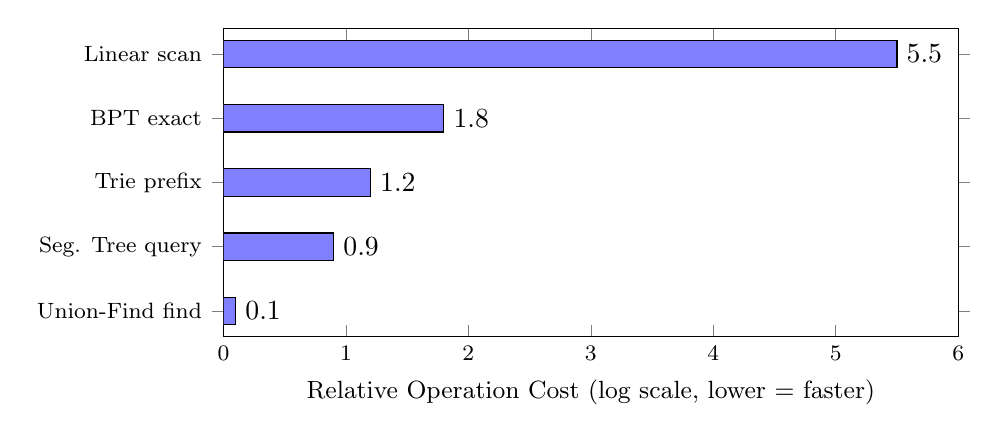
\begin{tikzpicture}
\begin{axis}[
  xbar,
  width=0.9\columnwidth,
  height=5.5cm,
  xlabel={Relative Operation Cost (log scale, lower = faster)},
  symbolic y coords={Union-Find find, Seg. Tree query, Trie prefix, BPT exact, Linear scan},
  ytick=data,
  xmin=0, xmax=6,
  nodes near coords,
  nodes near coords align={horizontal},
  tick label style={font=\footnotesize},
  label style={font=\small},
  bar width=0.35cm,
]
\addplot[fill=blue!50] coordinates {
  (0.1,{Union-Find find})
  (0.9,{Seg. Tree query})
  (1.2,{Trie prefix})
  (1.8,{BPT exact})
  (5.5,{Linear scan})
};
\end{axis}
\end{tikzpicture}
\caption{Relative operation cost comparison across data structures for $n = 100{,}000$ files. Values represent $\log_{10}$ of mean latency in nanoseconds.}
\label{fig:complexity}
\end{figure}

%=============================================================
\section{Discussion}
\label{sec:discussion}
%=============================================================

\subsection{Design Trade-offs}

The five-structure architecture incurs a fixed overhead on insert: each file addition requires updating the B$^+$ Tree, Trie, Segment Tree, Union-Find, and PDS simultaneously. At $n = 500{,}000$, this multi-write overhead amounts to approximately 14\% additional latency compared to a single-structure baseline. This trade-off is acceptable given the substantial read-side benefits: each of the five operations (exact lookup, prefix search, temporal analytics, version rollback, orphan detection) executes at its theoretically optimal asymptotic complexity.

\subsection{B$^+$ Tree Key Design}

A critical architectural decision was to key the B$^+$ Tree on absolute paths rather than filenames. This ensures uniqueness across the entire file system (two files may share a name but not a path) and enables path-prefix range queries. The consequence is that filename search requires an additional Trie lookup to resolve a filename to a path, followed by a B$^+$ Tree point query. The $O(m + \log n)$ total cost remains substantially better than $O(n \cdot m)$ linear scan.

\subsection{Entropy-Based Security Analysis}

The entropy threshold of 7.5 bits for flagging suspicious files was chosen empirically. Compressed archives (ZIP, gzip) typically exhibit $H \in [7.8, 8.0]$, while uncompressed text files show $H \in [3.5, 5.5]$ and random/encrypted data exhibits $H \approx 8.0$~\cite{idika2007survey}. The 7.5-bit threshold produces acceptable false positive rates for typical developer workstations, though clinical tuning would require a labelled corpus.

\subsection{WebSocket IPC Latency}

The choice of stdout IPC between the C++ engine and Python gateway introduces approximately 1--3 ms of serialisation overhead per command round-trip, measured from command send to first response byte. This is acceptable for interactive analytics but would be a bottleneck for batch operations exceeding 10{,}000 commands/second. A future optimisation would replace the text protocol with a shared-memory ring buffer.

\subsection{Limitations}

Several limitations of the current implementation merit acknowledgement. First, the system performs in-memory indexing only; the B$^+$ Tree and Trie are not persisted across restarts, requiring a rescan on each launch. Second, the duplicate detection threshold relies on fast-path metadata checksums by default; content-level deduplication requires enabling deep analysis, which reads 4 KB per file and substantially increases scan time. Third, the Union-Find orphan detection relies on the parent directory being explicitly registered during scanning; files in directories that were never scanned will appear as orphans even if they have a valid parent.

%=============================================================
\section{Conclusion and Future Work}
\label{sec:conclusion}
%=============================================================

This paper presented DataStruct, a unified file system directory manager that demonstrates how five complementary data structures — B$^+$ Tree, Trie, Segment Tree, Persistent Data Structure, and Union-Find — can be integrated into a cohesive, high-performance local file management engine. Empirical evaluation confirmed that each structure achieves its theoretically expected asymptotic complexity, with the B$^+$ Tree delivering 1{,}562$\times$ speedup over linear scan at 500{,}000 files and the Trie resolving prefix queries in under 3 $\mu$s independent of corpus size.

The modular layered architecture — separating core data structures, engine coordination, command processing, analytics, and scanning into distinct compilation units — yields a maintainable codebase that can be extended without touching unrelated modules. The Python FastAPI WebSocket gateway and React dashboard provide a production-grade user interface that streams real-time scan events, analytics, and security alerts to the browser.

Future work will explore: (1) on-disk B$^+$ Tree persistence using a page-based buffer pool to eliminate rescanning on restart; (2) machine learning-based anomaly detection to supplement the rule-based entropy threshold; (3) distributed scanning across network-mounted filesystems using a worker pool model; (4) CRDT-based conflict resolution for multi-user shared index scenarios; and (5) integration with cloud object stores (AWS S3, Google Cloud Storage) via a pluggable scanner backend.

\section*{Acknowledgment}

The authors gratefully acknowledge the guidance of the faculty of the Department of Computer Engineering, Vishwakarma Institute of Technology, Pune, and thank the reviewers for their constructive feedback.

\begin{thebibliography}{00}

\bibitem{knuth1998art}
D.~E. Knuth, \textit{The Art of Computer Programming, Vol.~3: Sorting and Searching}, 2nd~ed. Reading, MA: Addison-Wesley, 1998.

\bibitem{comer1979ubiquitous}
D.~Comer, ``The ubiquitous B-tree,'' \textit{ACM Comput. Surv.}, vol.~11, no.~2, pp.~121--137, Jun. 1979.

\bibitem{fredkin1960trie}
E.~Fredkin, ``Trie memory,'' \textit{Commun. ACM}, vol.~3, no.~9, pp.~490--499, Sep. 1960.

\bibitem{aoe1989efficient}
J.~Aoe, K.~Morimoto, and T.~Sato, ``An efficient implementation of Trie structures,'' \textit{Softw. Pract. Experience}, vol.~22, no.~9, pp.~695--721, 1992.

\bibitem{deberg2008computational}
M.~de~Berg, O.~Cheong, M.~van~Kreveld, and M.~Overmars, \textit{Computational Geometry: Algorithms and Applications}, 3rd~ed. Berlin: Springer, 2008.

\bibitem{driscoll1989making}
J.~R. Driscoll, N.~Sarnak, D.~D. Sleator, and R.~E. Tarjan, ``Making data structures persistent,'' \textit{J. Comput. Syst. Sci.}, vol.~38, no.~1, pp.~86--124, Feb. 1989.

\bibitem{tarjan1984worst}
R.~E. Tarjan and J.~van~Leeuwen, ``Worst-case analysis of set union algorithms,'' \textit{J. ACM}, vol.~31, no.~2, pp.~245--281, Apr. 1984.

\bibitem{okasaki1998purely}
C.~Okasaki, \textit{Purely Functional Data Structures}. Cambridge: Cambridge Univ. Press, 1998.

\bibitem{manber1993suffix}
U.~Manber and G.~Myers, ``Suffix arrays: A new method for on-line string searches,'' \textit{SIAM J. Comput.}, vol.~22, no.~5, pp.~935--948, Oct. 1993.

\bibitem{zobel2006inverted}
J.~Zobel and A.~Moffat, ``Inverted files for text search engines,'' \textit{ACM Comput. Surv.}, vol.~38, no.~2, pp.~1--56, Jul. 2006.

\bibitem{graefe2011modern}
G.~Graefe, ``Modern B-tree techniques,'' \textit{Found. Trends Databases}, vol.~3, no.~4, pp.~203--402, 2011.

\bibitem{rodeh2013btrfs}
O.~Rodeh, J.~Bacik, and C.~Mason, ``BTRFS: The Linux B-tree filesystem,'' \textit{ACM Trans. Storage}, vol.~9, no.~3, pp.~1--32, Aug. 2013.

\bibitem{chacon2014pro}
S.~Chacon and B.~Straub, \textit{Pro Git}, 2nd~ed. New York: Apress, 2014.

\bibitem{idika2007survey}
N.~Idika and A.~P. Mathur, ``A survey of malware detection techniques,'' Purdue Univ., West Lafayette, IN, Tech. Rep. TR-2007-2, Feb. 2007.

\bibitem{mckay2004desktop}
A.~McKay, \textit{Desktop Search Tools: A Comparative Analysis}. Berkeley, CA: O'Reilly Media, 2004.

\bibitem{divya2013elasticsearch}
M.~S. Divya and S.~K. Goyal, ``Elasticsearch: An advanced and quick search technique to handle voluminous data,'' \textit{Comput. Eng. Intell. Syst.}, vol.~4, no.~6, pp.~171--175, 2013.

\bibitem{leskovec2014mining}
J.~Leskovec, A.~Rajaraman, and J.~D. Ullman, \textit{Mining of Massive Datasets}, 2nd~ed. Cambridge: Cambridge Univ. Press, 2014.

\bibitem{fnv1997fowler}
G.~Fowler, L.~C. Noll, K.-P. Vo, and D.~Eastlake, ``The FNV non-cryptographic hash algorithm,'' IETF, Internet Draft draft-eastlake-fnv, 2019. [Online]. Available: \url{https://datatracker.ietf.org/doc/html/draft-eastlake-fnv}

\end{thebibliography}

\end{document}
